\section*{Problema 9}

\textbf{Se elige al azar un punto (X, Y ) adentro del siguiente triángulo. Calcula Cov(X, Y ).}

\begin{figure}[H]
    \centering
    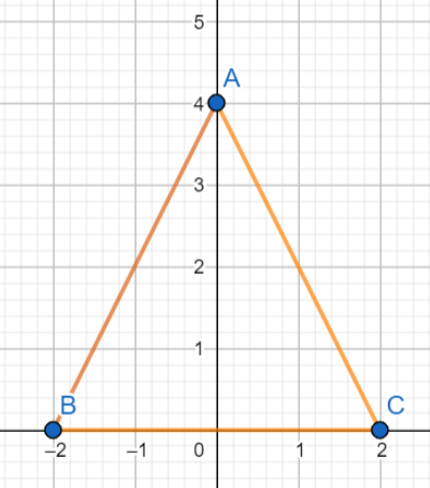
\includegraphics[width=3cm]{Graphics/problem9_image.png}
\end{figure}

Se tiene que la densidad de probabilidad conjunta es:

\begin{equation*}
    f(x,y) = \begin{cases}
        \frac{1}{8} & -2\leq x \leq 2 , 0\leq y \leq -2|x|+4 \\
        0           & c.o.p
    \end{cases}
\end{equation*}

Se tiene que

\begin{equation*}
    Cov(X,Y) = EXY -EX EY
\end{equation*}

Calculando $EXY$

\begin{align*}
    EXY & = \int\limits_{-2}^2 \int\limits_{0}^{-2|x|+4} \frac{xy}{8}dydx                                                                       \\
        & = \int\limits_{-2}^2 \frac{x}{8}\left (\frac{1}{2}(-2|x|+4)^2\right )                                                                 \\
        & = \int\limits_{-2}^0 \frac{x}{8}\left (\frac{1}{2}(2x+4)^2\right ) + \int\limits_{0}^2 \frac{x}{8}\left (\frac{1}{2}(-2x+4)^2\right ) \\
        & = -\frac{1}{3} + \frac{1}{3}                                                                                                          \\
    EXY & = 0
\end{align*}

Calculando $EX$

\begin{align*}
    EX & =  \int\limits_{-2}^2 \int\limits_{0}^{-2|x|+4} \frac{x}{8}dydx                   \\
       & =  \int\limits_{-2}^2 \frac{x}{8}(-2|x|+4)dx                                      \\
       & = \int\limits_{-2}^0 \frac{x}{8}(2x+4)dx + \int\limits_{0}^2 \frac{x}{8}(-2x+4)dx \\
       & = -\frac{1}{3} + \frac{1}{3}                                                      \\
    EX & = 0
\end{align*}

como $EX=0$, ya no es necesaio calcular $EY$, ya que $0(EY)=0$, por lo tanto:

\begin{equation*}
    Cov(X,Y) = 0
\end{equation*}